% Relatório da versão 1 do software ipump para o curso
% Sistemas de Controle - DCA0206 - UFRN
% Autores:
%   AUGUSTO MATHEUS PINHEIRO DAMASCENO
%   MARCEL DA CÂMARA RIBEIRO DANTAS
%   PABLO HOLANDA CARDOSO
%   PEDRO DE CASTRO GURGEL LIMA
%   RODRIGO DANTAS DA SILVA
% Modificado por: Ícaro Bezerra Queiroz de Araújo
%

%%%%%%%%%%%% STRUCTURE %%%%%%%%%%%%%%%
\documentclass[a4paper,12pt]{article}
\usepackage[T1]{fontenc}
\usepackage[utf8]{inputenc}
\usepackage[brazil]{babel}
\usepackage{lmodern}
\usepackage{setspace}
\usepackage[top=2cm, bottom=2cm, left=2cm, right=2cm]{geometry}
%%%%%%%%%%%%%%%%%%%%%%%%%%%%%%%%%%%%%%

%%%%%%%%%%%%%%%% PAGES STYLE %%%%%%%%%
\usepackage{fancyhdr}
\fancypagestyle{main}{
\renewcommand{\headrulewidth}{0pt}
\fancyhead[RO]{\thepage}
\fancyfoot[CO]{}
}
%%%%%%%%%%%%%%%%%%%%%%%%%%%%%%%%%%%%%%

\usepackage{graphicx}
\usepackage{float}
\usepackage{epstopdf}
\usepackage{subfig}
\usepackage{mathptmx}
\usepackage{changepage}


\usepackage{listings}
\usepackage{xcolor}
\lstset{language=C++,
                basicstyle=\ttfamily,
                keywordstyle=\color{blue}\ttfamily,
                stringstyle=\color{red}\ttfamily,
                commentstyle=\color{green}\ttfamily,
                morecomment=[l][\color{magenta}]{\#}
}

%\usepackage[alf]{abntex2cite}

%%%%%%%%%%% PDF METADATA %%%%%%%%%%%%%
\usepackage[ pdftitle={MODELO RELATÓRIO},
pdfsubject={INTRODUÇÃO AO LABORATÓRIO DE CONTROLE - Grupo 3},
pdfkeywords={Controle,Automação,UFRN,DCA,ipump},
hidelinks]{hyperref}
%%%%%%%%%%%%%%%%%%%%%%%%%%%%%%%%%%%%%%

\begin{document}

\onehalfspacing

\thispagestyle{empty}

\setcounter{page}{1}

%%%%%%%%%%%% LOGOS %%%%%%%%%%%%%%%%%%%

\begin{figure}[!ht]

\centering

\subfloat{

\includegraphics[width=2.7cm]{UFRN.eps}
\label{UFRN Logo}
}
\hspace{11.09cm}
\subfloat{

\includegraphics[width=2.4cm]{DCA.eps}
\label{DCA Logo}
}

%\caption{}
\label{Logos}

\end{figure}

%%%%%%%%%%%%%%% CAPA %%%%%%%%%%%%%%%%%

\vspace{-1cm}

\begin{center}
{\bf{\normalsize UNIVERSIDADE FEDERAL DO RIO GRANDE DO NORTE\\
CENTRO DE TECNOLOGIA\\
DEPARTAMENTO DE ENGENHARIA DE COMPUTAÇÃO E AUTOMAÇÃO\\
CURSO DE ENGENHARIA DE COMPUTAÇÃO
}}


\vspace{3.6cm}

{\bf{\large RELATÓRIO DA 6ª EXPERIÊNCIA\\
CONTROLE NO ESPAÇO DE ESTADOS: SEGUIDOR DE REFERÊNCIA\\
}}
\vspace{1.5cm}
{\large TURMA: 01 A\\
	GRUPO Nº 02}


\vspace{3.6cm}


\begin{flushright}
\begin{normalsize}
ANDRESSA STÉFANY SILVA DE OLIVEIRA: 20160154101\\
\vspace{0.8cm}
FERNANDA MONTEIRO DE ALMEIDA: 20160154228\\
\vspace{0.8cm}
MÁRCIO LUIZ BEZERRA LOPES JÚNIOR: 20160154326\\
\vspace{0.8cm}
VITOR RAMOS GOMES DA SILVA: 20160154415\\
\end{normalsize}
\end{flushright}


\vspace{2.5cm}

{\large Natal-RN\\
2017}

\end{center}

\newpage

%%%%%%%%%%%%%%%  CONTRA-CAPA %%%%%%%%%

\thispagestyle{empty}

\begin{center}
\begin{normalsize}
ANDRESSA STÉFANY SILVA DE OLIVEIRA: 2016015410\\
\vspace{0.8cm}
FERNANDA MONTEIRO DE ALMEIDA 20160154228\\
\vspace{0.8cm}
MÁRCIO LUIZ BEZERRA LOPES JÚNIOR: 20160154326\\
\vspace{0.8cm}
VITOR RAMOS GOMES DA SILVA: 20160154415\\

\end{normalsize}
\end{center}
\vspace{3cm}

{\bf{\large {\centering CONTROLE NO ESPAÇO DE ESTADOS: SEGUIDOR DE REFERÊNCIA\\}}}

\vspace{4cm}

\begin{adjustwidth}{7.5cm}{0cm}

{\normalsize
Sexto relatório apresentado à disciplina de
Laboratório de Sistemas de Controle, correspondente à
avaliação da 3º unidade do semestre 2017.1 do 8º período
do curso de Engenharia de Computação da
Universidade Federal do Rio Grande do Norte, sob
orientação do {\bf Prof. Fábio Meneghetti Ugulino de
Araújo} e {\bf Prof. Lucas Costa Pereira Cavalcante.}

}

\end{adjustwidth}

\vspace{2cm}

\begin{center}

Professores:  Fábio Meneghetti Ugulino de Araújo e\\
Lucas Costa Pereira Cavalcante.

\vspace{2.5cm}

{\large Natal-RN\\
2017}

\end{center}

\newpage

%%%%%%%%%%%%%%%  RESUMO %%%%%%%%%%%%%%

\thispagestyle{empty}

\begin{center}
{\large \textbf{RESUMO}}
\end{center}

\vspace{3cm}

\begin{flushleft}

\hspace{4ex}O presente trabalho é a sexta etapa da construção de um aplicativo desktop para controle de sistema de tanques. O software utiliza a comunicação cliente/servidor no qual o sistema de tanques é o servidor. A planta antes utilizada da Quanser foi substituída por uma simulação feita em Java3D, o que eliminou o nível de ruído dos resultados. Nesta etapa do trabalho, o objetivo foi projetar e implementar um seguidor de referência para um controlador proporcional de segunda ordem. A teoria acerca do seguidor de referência  é introduzida, após são apresentados os resultados dos testes de controle da planta. Por fim, chega-se a conclusão que a aproximação do pólo em zero torna o sistema instável, e que este responde agressivamente a pólos com grande parte imaginária. \\

\end{flushleft}

\vspace{1.5cm}

\textbf{Palavras-chave:} sistema de tanques; sistema de controle; software; planta Quanser, controlador PID; espaço de estados, seguidor de referência.

\newpage

%%%%%%%%% LISTA DE FIGURAS %%%%%%%%%%%

\thispagestyle{empty}

\begin{center}
\listoffigures
\end{center}

\newpage

%%%%%%%%%%%%%%% SUMÁRIO %%%%%%%%%%%%%%

\thispagestyle{empty}

\begin{center}
\tableofcontents
\end{center}

\newpage

%%%%%%%%%%%%%%% INTRODUÇÃO %%%%%%%%%%%

\thispagestyle{main}

\section{INTRODUÇÃO}

%\begin{flushleft}
\hspace{4ex}A prática de laboratório 06 tem como objetivo introduzir o conceito de seguidor de referência. Nesse relatório será apresentado a implementação de um seguidor de referência discreto para controlar o nível do tanque de baixo da planta \textit{Quanser}, sendo a figura \ref{r2d2e} a representação do simulador da planta:

\begin{figure}[H]
\centering
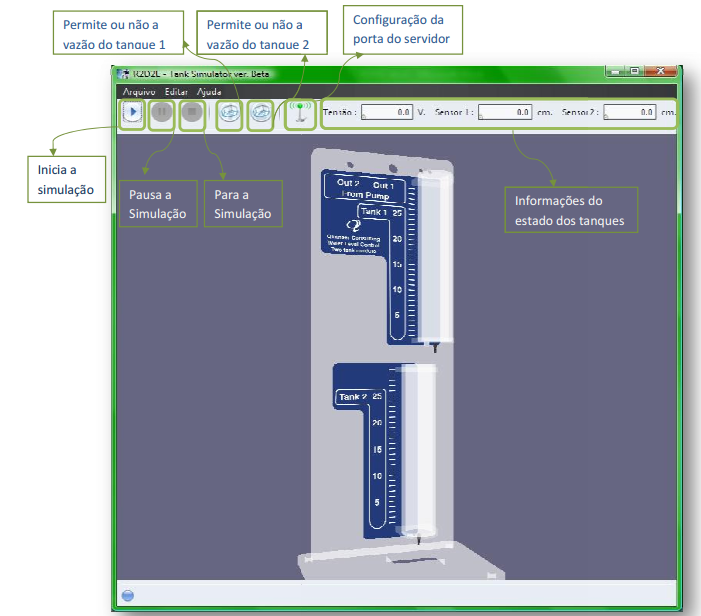
\includegraphics[width=11cm]{ImagensLab4/simulator.png}
\caption{R2D2E - Tank Simulator}
\label{r2d2e}
\end{figure}

\hspace{4ex}Essa planta é controlada através de um software desenvolvido, o qual disponibiliza opção de controle em malha aberta e malha fechada. Em malha aberta, o usuário informa a tensão que quer enviar para bomba que encherá o tanque, enquanto que em malha fechada, o valor informado será o nível do tanque. Além disso, em malha fechada, também deverá ser informado a ordem do sistema, ou seja, se o objetivo é controlar apenas o tanque de cima($L_1$) ou se o desejado é o controle do tanque de baixo($L_2$), onde nesse último caso é usado o controle em cascata. Com isso, há as opções de controle utilizando os controladores Proporcional (P), Proporcional Integrativo (PI), Proporcional Derivativo (PD), Proporcional Integrativo Derivativo (PID) e Proporcional Integrativo Derivativo em controle de ação baseado no sinal do processo (PI-D). Uma outra opção disponível é o observador de estados, sendo necessário informar a matriz de ganhos ou os pólos desejados para o observador.

\hspace{4ex}Nesse laboratório, foi adicionado mais uma opção de controle: o usuário poderá controlar o sistema, o qual será utilizado o sistema de segunda ordem em malha fechada, usando um seguidor de referência para entradas do tipo degrau.

\hspace{4ex}Na interface do software desenvolvido, o usuário deverá informar quais serão os valores dos pólos ou informar os ganhos do seguidor de referência, observe a figura \ref{interface}.

\begin{figure}[H]
\centering
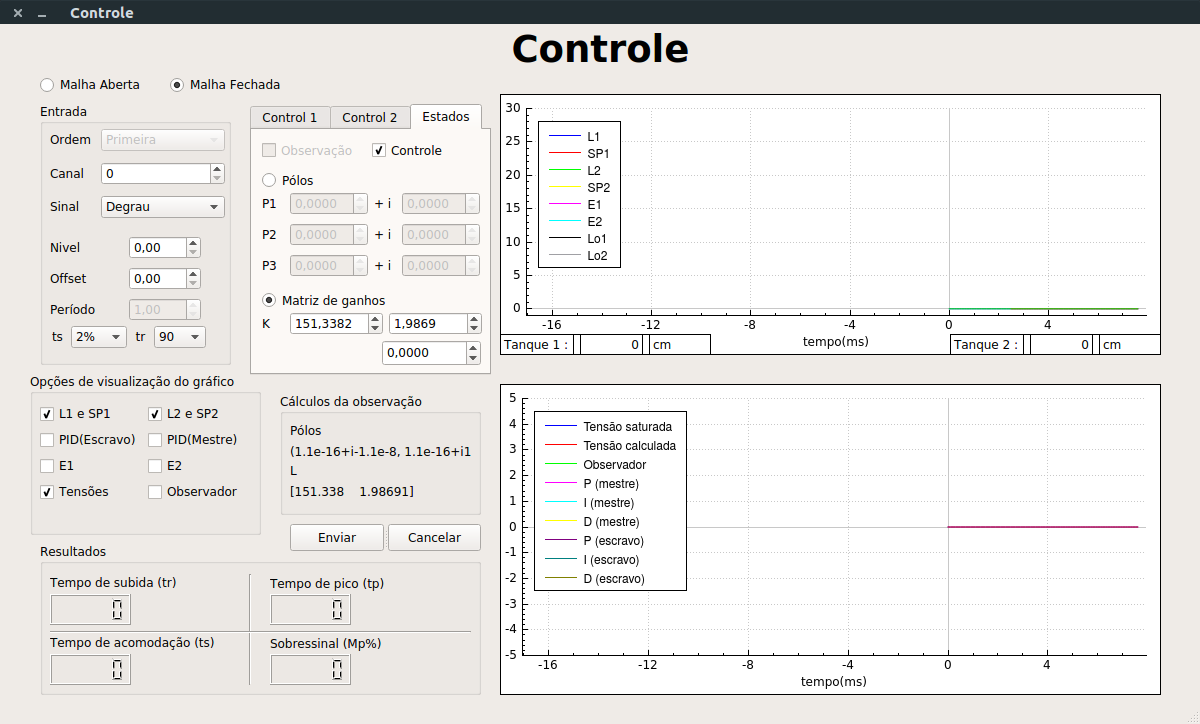
\includegraphics[width=13cm]{FotosSeguidor/telaRef.png}
\caption{Interface do software de controle}
\label{interface}
\end{figure}

\hspace{4ex}Mais à frente, será abordado no relatório em que os cálculos foram baseados para a obtenção do seguidor de referência, a metodologia utilizada no trabalho, como também será apresentado o comportamento do controlador para diferentes conjuntos de pólos e, por conseguinte, a conclusão a cerca desse controle.

%\end{flushleft}

\newpage

%%%%%%%%%% REFERENCIAL TEÓRICO %%%%%%%

\thispagestyle{main}

\section{REFERENCIAL TEÓRICO}

\subsection{SISTEMA DISCRETO NO TEMPO}

\hspace{4ex}Dado um sistema linear discreto invariante no tempo descrito pelas variáveis de estado:

\begin{figure}[H]
\centering
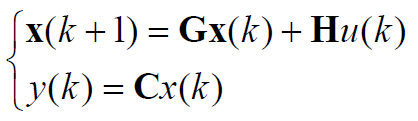
\includegraphics[width=5cm]{imagens-6/1.png}
\end{figure}


A representação discreta de um sistema será obtido, a partir de sua representação contínua, por:
\begin{figure}[H]
\centering
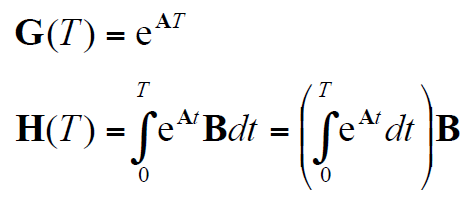
\includegraphics[width=5cm]{imagens-6/18.png}
\end{figure}


\subsubsection{ESTABILIDADE}
Dado:
\begin{figure}[H]
\centering
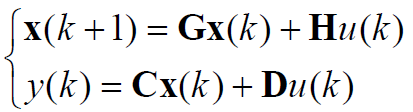
\includegraphics[width=5cm]{imagens-6/19.png}
\end{figure}
Um sistema de estados discreto será considerado estável caso todos os autovalores da matriz \textbf{G} estejam localizados dentro do círculo unitário.

\subsubsection{CONTROLABILIDADE}
Um sistema de estados discreto será considerado controlável se sua matriz de controlabilidade (nxn) tiver posto n.

\begin{figure}[H]
\centering
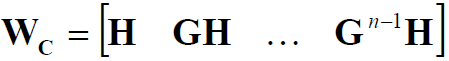
\includegraphics[width=5cm]{imagens-6/20.png}
\caption{Matriz de Controlabilidade}
\end{figure}

\subsubsection{OBSERVABILIDADE}
Um sistema de estados discreto será considerado observável se sua matriz de observabilidade (nxn) tiver posto n.

\begin{figure}[H]
\centering
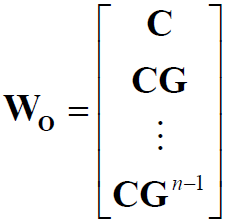
\includegraphics[width=3cm]{imagens-6/21.png}
\caption{Matriz de Observabilidade}
\end{figure}

\subsection{SEGUIDOR DE REFERÊNCIA}
\hspace{4ex}Seguidores de referência, ou servosistemas, são sistemas descritos por variáveis de estado projetados para, além de ter uma dinâmica desejada, seguir uma entrada especificada, de erro zero. Para projetar sistemas deste tipo, é usado o princípio do modelo interno, que diz que um sistema em malha fechada irá seguir um sinal de referência de entrada, sem erro em regime permanente, quando o modelo que gera esta referência estiver incluso no sistema realimentado estável.

\subsection{PROJETO DE SEGUIDOR DISCRETO}

\hspace{4ex}Considerando um sistema discreto no tempo:
\begin{figure}[H]
\centering
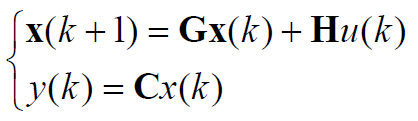
\includegraphics[width=5cm]{imagens-6/1.png}
\end{figure}


Com um sinal:
\begin{figure}[H]
\centering
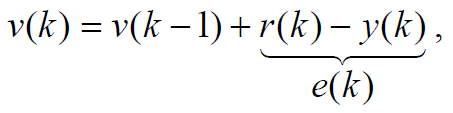
\includegraphics[width=5cm]{imagens-6/2.png}
\end{figure}


E sendo:
\begin{figure}[H]
\centering
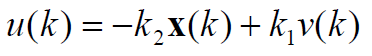
\includegraphics[width=5cm]{imagens-6/4.png}
\end{figure}


É possível através de substituições e do desenvolvimento das equações, encontrar:
\begin{figure}[H]
\centering
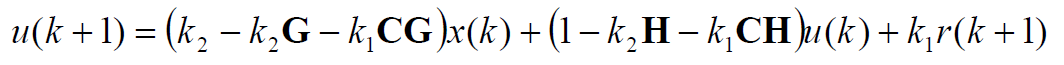
\includegraphics[width=12cm]{imagens-6/5.png}
\end{figure}


A partir do qual, tem-se:
\begin{figure}[H]
\centering
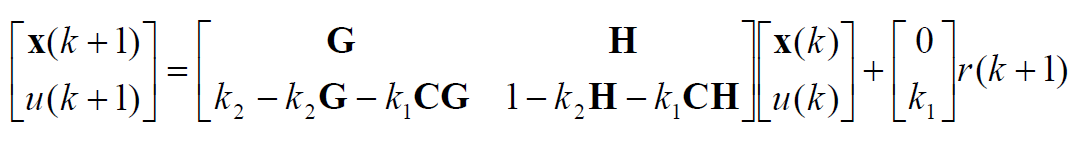
\includegraphics[width=12cm]{imagens-6/7.png}
\end{figure}


Para o caso dos autovalores da matriz acima serem estáveis, com  k tendendo ao infinito:
\begin{figure}[H]
\centering
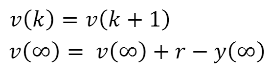
\includegraphics[width=5cm]{imagens-6/14.png}
\end{figure}

\break


Considerando a referência do \textbf{tipo degrau} e definindo:
\begin{figure}[H]
\centering
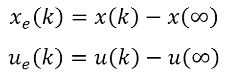
\includegraphics[width=4cm]{imagens-6/15.png}
\end{figure}


Tem-se que:
\begin{figure}[H]
\centering
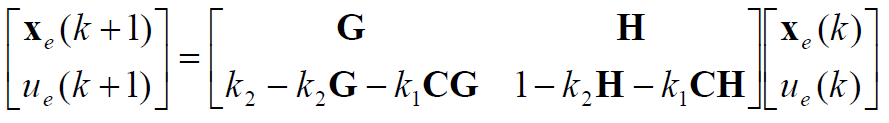
\includegraphics[width=9cm]{imagens-6/10.png}
\end{figure}


Definindo w(k):
\begin{figure}[H]
\centering
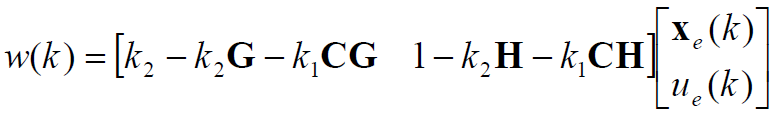
\includegraphics[width=9cm]{imagens-6/11.png}
\end{figure}


Encontra-se:
\begin{figure}[H]
\centering
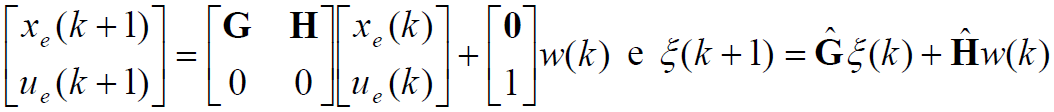
\includegraphics[width=10cm]{imagens-6/12.png}
\end{figure}


Sendo a alimentação de estados:
\begin{figure}[H]
\centering
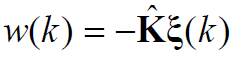
\includegraphics[width=3cm]{imagens-6/16.png}
\end{figure}


E conhecendo Fórmula de Ackermann para controle discreto:
\begin{figure}[H]
\centering
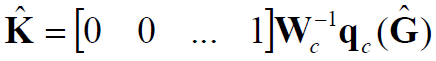
\includegraphics[width=5cm]{imagens-6/17.png}
\end{figure}


Finalmente, acha-se o modelo para o seguidor de referência desejado:
\begin{figure}[H]
\centering
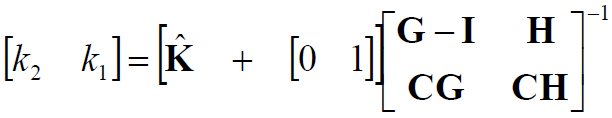
\includegraphics[width=7cm]{imagens-6/13.png}
\end{figure}


\newpage

%%%%%%%%%% METODOLOGIA %%%%%%%%%%%%%%%



\section{METODOLOGIA}

\hspace{4ex}Para o seguidor de referência, foi necessário obter as matrizes G aumentada e H aumentada, a partir do sistema discreto calculado na experiência anterior. Tais matrizes foram utilizadas para o cálculo da matriz de ganhos K.
%%matrizes
%\[
%G_A = 
%\begin{matrix}
%0.993452 & 0        & 0.0295461 \\ 
%0.006521 & 0.993457 & 0.0000968713 \\ 
%0        & 0        & 0
%\end{matrix} 
%\]

O programa desenvolvido oferece duas opções de entrada para o seguidor de referência: o primeiro, os pólos para se encontrar os ganhos; ou entrar com os ganhos. Para o caso em que os ganhos forem oferecidos, o programa calcula os pólos referentes àqueles ganhos.

\hspace{4ex}Uma vez com as informações importantes do sistema, a implementação do seguidor se resume nos seguintes métodos.

\begin{lstlisting}

double Seguidor::Seguir(Matriz x, Matriz r)
{
    erro+=r[0][0]-x[1][0];
    return -K[0][0]*x[0][0]-K[0][1]*x[1][0]+K[0][2]*(erro);
}

Matriz Seguidor::Calcula_K(complex<double> p1, complex<double> p2, complex<double> p3)
{
    Matriz I= Matriz::Identidade(3), aux(1,3);
    aux= {{0,0,1}};
    double c[3]= {(-p1-p2-p3).real(), (p1*p2+p2*p3+p1*p3).real(),(-p1*p2*p3).real()};
    Matriz Ackerman= (Ga^3)+(Ga^2)*c[0]+Ga*c[1]+I*c[2];
    K= aux*W_inv*Ackerman;
    K= (K+aux)*Kaux;
    return K;
}

\end{lstlisting}

\hspace{4ex}Os métodos acima, são algoritmos que representam os cálculos citados no referencial teórico. Já no método para encontrar os pólos, foi feito uma manipulação algébrica a partir das equações para encontrar a matriz K.

\hspace{4ex}A interface para entrada de dados do usuário se assemelha ao que foi feito para o observador. Porém, foi feito alterações para melhorar a experiência do usuário. Retirou-se da entrada do ganho $K_p$ pois era redudante e acrescentou-se mais um elemento na matriz de ganho, devido ao sistema aumentado. 

\begin{figure}[H]
     \centering
     \subfloat[]{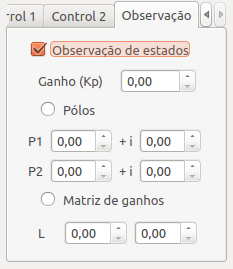
\includegraphics[width=6.65cm]{fotosLab5/observador-interface.png}\label{interface-obs}}    
\hspace{1cm}
     \subfloat[]{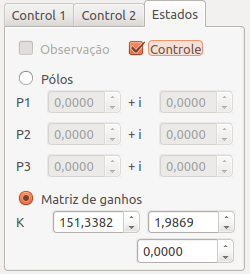
\includegraphics[width=7cm]{imagens-6/interface.png}\label{interface-ctl}}
     
     \caption{Comparação entre versões}
     \label{fig:interface-in}
\end{figure}

\hspace{4ex}Por fim, utilizando o simulador R2D2E, foram feitos testes de controle fixado no tipo proporcional para o sistema de segunda ordem com apenas um controlador. Sendo que o foco foi o teste com vários pólos, pois desejava-se encontrar os pólos mais adequados para o sistema. 




\newpage

%%%%%%%%%% RESULTADOS %%%%%%%%%%%%%%%

\thispagestyle{main}

\section{RESULTADOS}
\hspace{4ex}Nas figuras a seguir será apresentado os gráficos da interface do software, a qual mostrará o comportamento do seguidor de referência para entradas do tipo degrau com vários pólos, onde a curva em azul indica o nível do tanque 1($L_1$) e a curva em verde é o nível do tanque 2($L_2$).

\hspace{4ex}Inicialmente, como mostrado nas figuras \ref{img1}, foram iseridos os pólos 0,9048; 0,9920; 0,9980, para esses pólos o sistema foi bastante lento, demorando mais de 200 segundos para chegar em uma faixa de 2\% do valor da referência.
\begin{figure}[H]
\centering
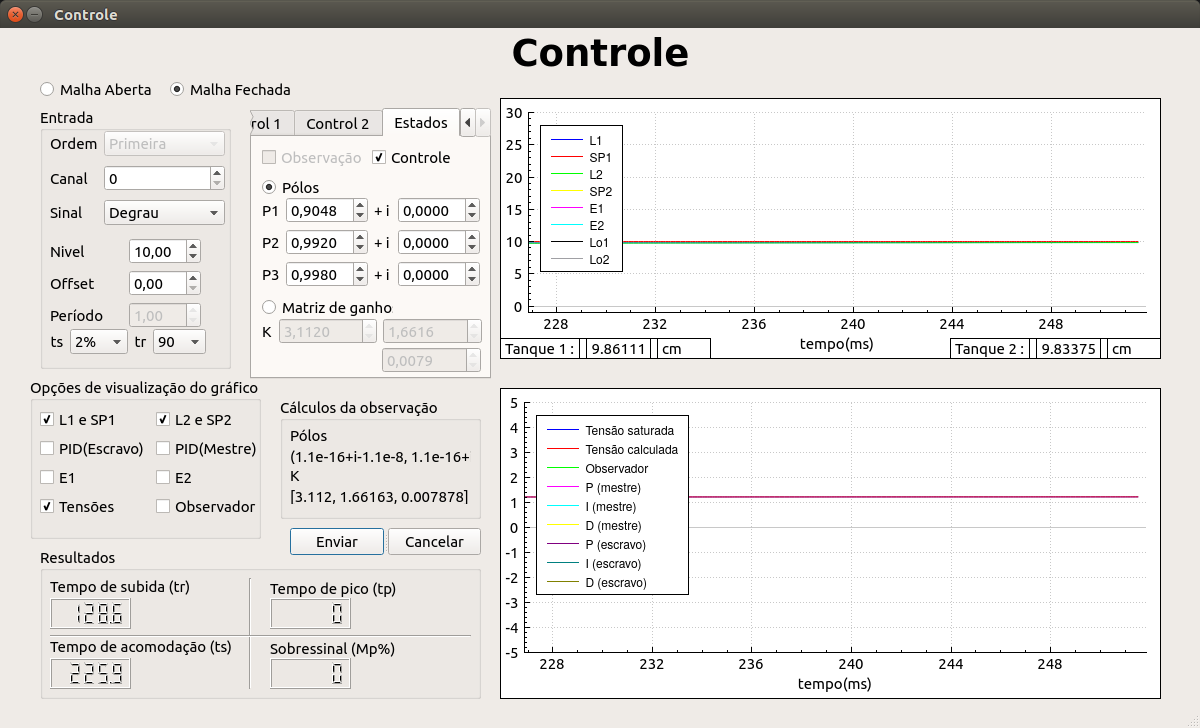
\includegraphics[width=13cm]{FotosSeguidor/PolosDados.png}
\caption{Seguidor}
\label{img1}
\end{figure}

\hspace{4ex}Agora com os pólos 0,9000; 0,9000; 0,9900; podemos ver na figura \ref{img3} que a resposta do sistema chegou na referência mais rapidamente.
\begin{figure}[!h]
\centering
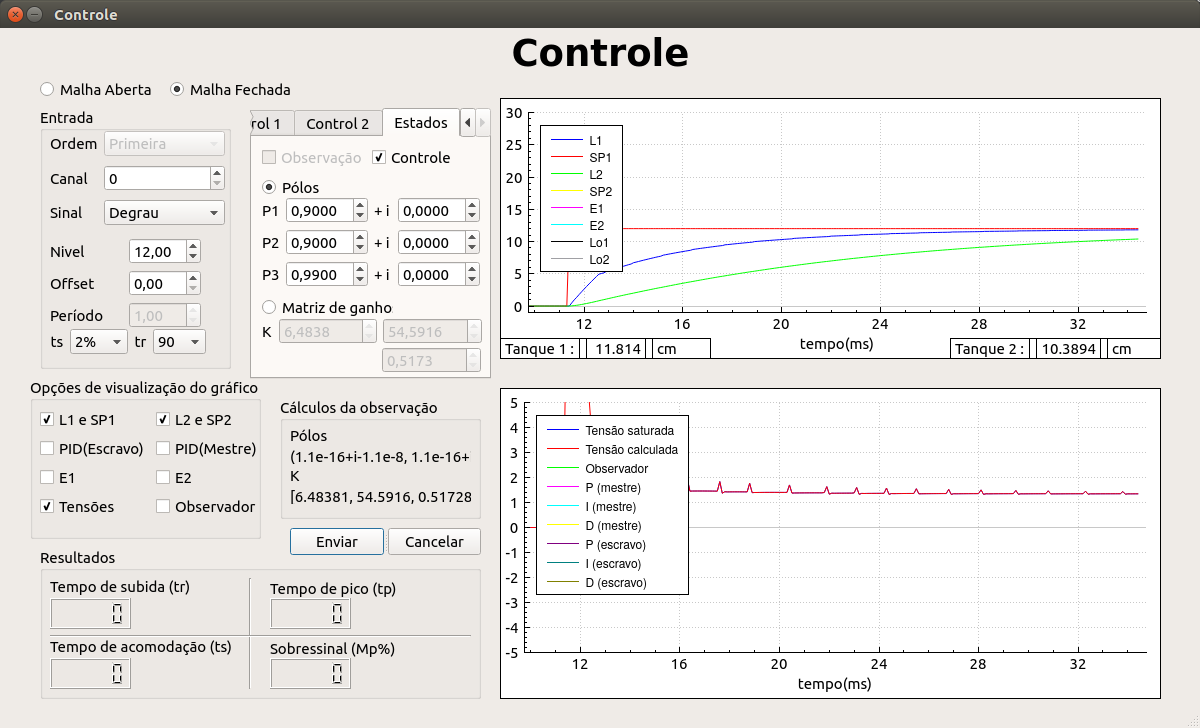
\includegraphics[width=13cm]{FotosSeguidor/Bom}
\caption{Seguidor}
\label{img3}
\end{figure}

\hspace{4ex}Com os pólos 0,9000; 0,9000; 0,9800; a resposta foi ainda mais rápida, isso pode ser notado na figura \ref{img4}.
\begin{figure}[!h]
\centering
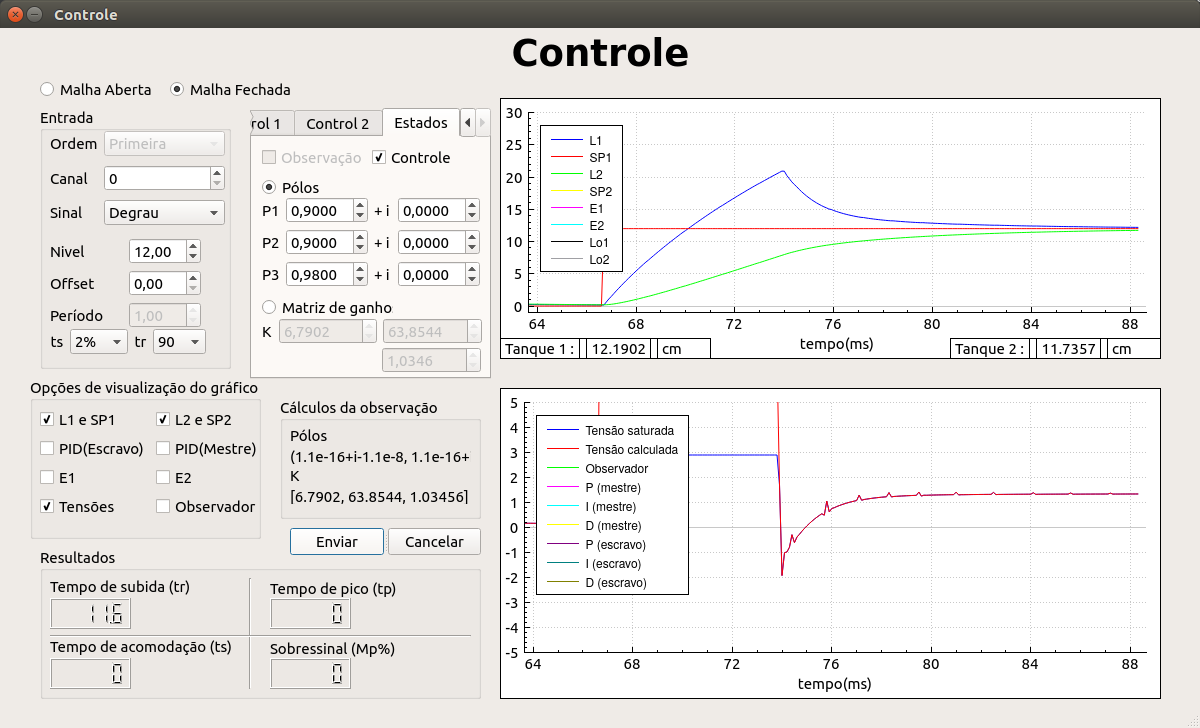
\includegraphics[width=13cm]{FotosSeguidor/MuitoBom}
\caption{Seguidor}
\label{img4}
\end{figure}


\hspace{4ex}Para os pólos imaginários, foi observado que o controlador fica bastante agressivo e, logo em seguida, fica instável, por isso foram utilizados valores pequenos para as partes imaginárias, como pode ser verificado nas figuras \ref{img5} e \ref{img6}.
\begin{figure}[!h]
\centering
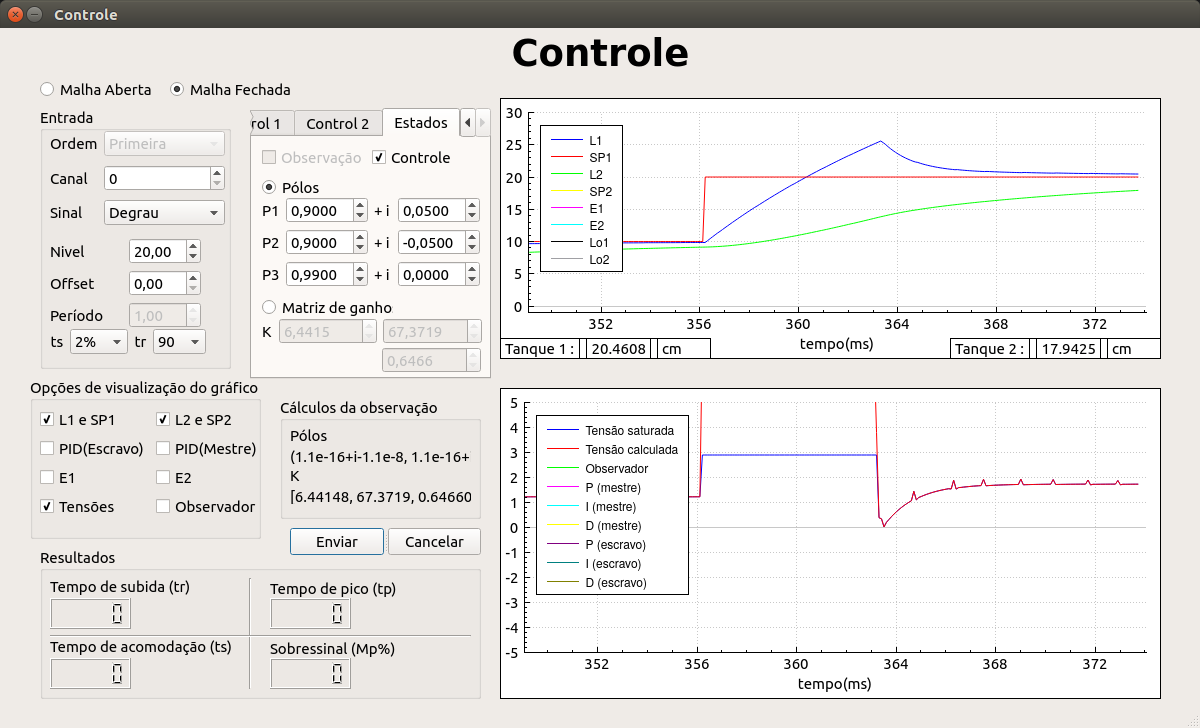
\includegraphics[width=13cm]{FotosSeguidor/PolosComplexos}
\caption{Seguidor}
\label{img5}
\end{figure}
\begin{figure}[!h]
\centering
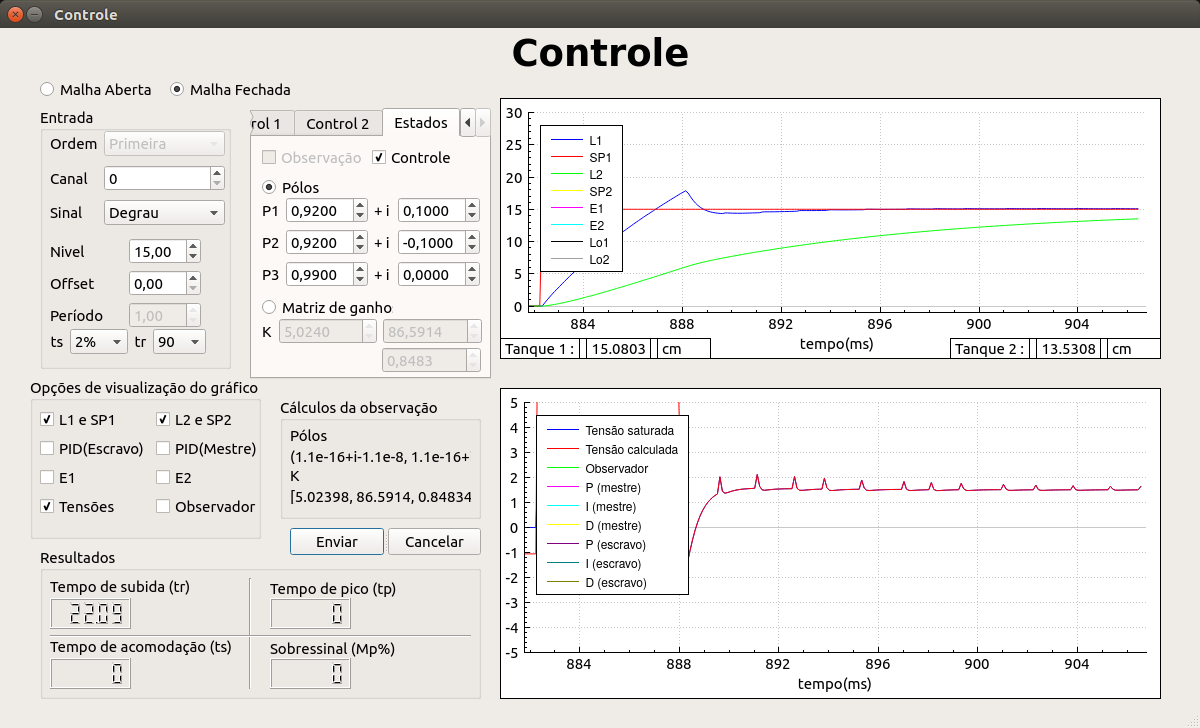
\includegraphics[width=13cm]{FotosSeguidor/PolosComplexos2}
\caption{Seguidor}
\label{img6}
\end{figure}

\newpage
.
\newpage
%%%%%%%%%% CONCLUSÃO %%%%%%%%%%%%%%%

\thispagestyle{main}

\section{CONCLUSÃO}

\hspace{4ex}A partir dos testes realizados com os pólos próximos do círculo unitário, sendo alguns com parte imaginária e outros não, pode-se concluir que o controle da planta realizado através do seguidor de referência torna o sistema instável à medida que o pólo vai se aproximando de zero e quando a parte imaginária do pólo é grande, isso também resulta em uma resposta de comportamento agressivo.

\newpage
%%%%%%%% REFERÊNCIAS %%%%%%%%%%%%%%%%%

\thispagestyle{empty}
\section{BIBLIOGRAFIA}

Fundamentals of cascade control | Control Engineering. Disponível em: <http://www.controleng.com/single-article/fundamentals-of-cascade-control/bcedad6518aec409f583ba6bc9b72854.html>. Acesso em: 10 maio. 2017.




%Referências bibliogáficas (geradas automaticamente)

%\addcontentsline{toc}{chapter}{Referências bibliográficas}
%\bibliography{bib/bibliografia}

%\appendix

%Apêndice A
%\include{apendice}

\end{document}
